% fig_architecture_hybridblock.tex
% Figure: HybridBlock internal structure
% Compact layout: tighter 0.75 cm node spacing, no output thumbnail,
% WindowAttnBlock label placed BELOW its group box (avoids ResBlock overlap).
% Outer residual routed on the RIGHT at x=+1.8 (clear of annotation panel).
\begin{figure}[htbp]
\centering
\resizebox{0.65\linewidth}{!}{%
\begin{tikzpicture}[
  >=Stealth,
  every node/.style={font=\small},
  imgblk/.style={inner sep=0pt, outer sep=0pt},
  fmblk/.style={inner sep=0pt, outer sep=0pt},
  rbbox/.style={draw=blue!60!black, fill=blue!10, rounded corners=3pt,
                minimum width=3.0cm, minimum height=0.75cm,
                align=center, line width=0.8pt},
  rbnorm/.style={draw=teal!65!black, fill=teal!9, rounded corners=3pt,
                 minimum width=3.0cm, minimum height=0.75cm,
                 align=center, line width=0.8pt},
  rbact/.style={draw=orange!65!black, fill=orange!9, rounded corners=3pt,
                minimum width=3.0cm, minimum height=0.75cm,
                align=center, line width=0.8pt},
  wabox/.style={draw=purple!60!black, fill=purple!9, rounded corners=3pt,
                minimum width=3.0cm, minimum height=0.75cm,
                align=center, line width=0.8pt},
  wanorm/.style={draw=teal!65!black, fill=teal!9, rounded corners=3pt,
                 minimum width=3.0cm, minimum height=0.75cm,
                 align=center, line width=0.8pt},
  waffn/.style={draw=orange!60!black, fill=orange!10, rounded corners=3pt,
                minimum width=3.0cm, minimum height=0.75cm,
                align=center, line width=0.8pt},
  addnode/.style={draw=gray!65, fill=gray!13, circle,
                  minimum size=0.55cm, align=center, line width=0.8pt,
                  font=\normalsize},
  groupbox/.style={draw=gray!50, fill=gray!4, rounded corners=5pt,
                   dashed, line width=1.0pt},
  dimtag/.style={font=\fontsize{7}{8}\selectfont, text=black!60, align=center},
  arrmain/.style={->, line width=1.5pt, black!70},
  arrskip/.style={->, line width=1.2pt, blue!70, dashed},
  arrwa/.style={->, line width=1.1pt, purple!65, dashed},
]

% ── Input ─────────────────────────────────────────────────────────
\node[dimtag] at (0,10.5) {$\mathbf{f}_{\mathrm{in}}$\;($H{\times}W{\times}C$)};
\node[imgblk] (fin_img) at (0,9.6)
  {\includegraphics[width=1.2cm,height=1.2cm,keepaspectratio]%
    {figures/arch/arch_input_noisy.png}};

% ── ResBlock (0.75 cm centre-to-centre) ───────────────────────────
\node[rbbox]  (rb_c1)  at (0,8.2)  {\textbf{Conv}\;$3{\times}3$,\;pad\;1};
\node[rbnorm] (rb_gn1) at (0,7.45) {\textbf{GroupNorm}\;($G{=}8$)};
\node[rbact]  (rb_g1)  at (0,6.7)  {\textbf{GELU}};
\node[rbbox]  (rb_c2)  at (0,5.95) {\textbf{Conv}\;$3{\times}3$,\;pad\;1};
\node[rbnorm] (rb_gn2) at (0,5.2)  {\textbf{GroupNorm}\;($G{=}8$)};
\node[addnode](rb_add) at (0,4.4)  {$+$};
\node[rbact]  (rb_g2)  at (0,3.65) {\textbf{GELU}};

% ResBlock group box (label above)
\begin{scope}[on background layer]
  \node[groupbox, inner sep=6pt,
        fit=(rb_c1)(rb_gn1)(rb_gn2)(rb_add)(rb_g2),
        label={[font=\fontsize{8}{9}\selectfont\bfseries,
                text=blue!70]above:\strut ResBlock}] (rbgroup) {};
\end{scope}

% ResBlock skip: fin_img.west → down left → rb_add.west
\draw[arrskip]
  (fin_img.west)
  -- ++(-1.4,0)
  -- node[left,font=\fontsize{7}{8}\selectfont,xshift=-2pt]{skip}
     ++(0,-5.2)
  -| (rb_add.west);

% ── f_res feature map ─────────────────────────────────────────────
\node[fmblk] (fm_res) at (-0.7,3.0)
  {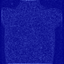
\includegraphics[width=0.72cm,height=0.72cm]{figures/arch/featmap_256.png}};
\node[dimtag,right=4pt of fm_res]
  {$\mathbf{f}_{\mathrm{res}}$\;($H{\times}W{\times}C$)};

% ── WindowAttnBlock ───────────────────────────────────────────────
\node[wanorm] (wa_ln1) at (0,2.1)   {\textbf{LayerNorm}};
\node[wabox]  (wa_mha) at (0,1.2)
  {\textbf{Multi-head Attention}\\
   {\fontsize{7}{8}\selectfont 4\;heads,\;$8{\times}8$\;windows}};
\node[wanorm] (wa_ln2) at (0,0.2)   {\textbf{LayerNorm}};
\node[waffn]  (wa_ffn) at (0,-0.7)
  {\textbf{FFN}\;{\fontsize{7}{8}\selectfont (Lin.\;$4C$--GELU--Lin.\;$C$)}};
\node[addnode](wa_add) at (0,-1.7)  {$+$};

% WindowAttnBlock group box (label BELOW to avoid ResBlock overlap)
\begin{scope}[on background layer]
  \node[groupbox, inner sep=6pt,
        fit=(wa_ln1)(wa_mha)(wa_ln2)(wa_ffn)(wa_add),
        label={[font=\fontsize{8}{9}\selectfont\bfseries,
                text=purple!65]below:\strut WindowAttnBlock}] (wagroup) {};
\end{scope}

% Outer residual: f_res level → right arm → wa_add.east
\draw[arrwa]
  (0,3.0)
  -- ++(1.8,0)
  -- node[left,font=\fontsize{6}{7}\selectfont,text=purple!70]
       {outer\\[-1pt]residual}
     ++(0,-4.7)
  -| (wa_add.east);

% f_out label
\node[dimtag] at (0,-2.5)
  {$\mathbf{f}_{\mathrm{out}}$\;($H{\times}W{\times}C$)};

% ── RIGHT PANEL: 8×8 window partition ────────────────────────────
\begin{scope}[shift={(2.6,-0.7)}]
  \node[fmblk] at (1.1,1.1)
    {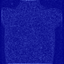
\includegraphics[width=2.2cm,height=2.2cm]{figures/arch/featmap_256.png}};
  \draw[white,line width=0.3pt,opacity=0.6,step=0.367] (0,0) grid (2.2,2.2);
  \draw[purple!80!white,line width=1.4pt,step=0.733] (0,0) grid (2.2,2.2);
  \draw[purple!80!white,line width=1.4pt] (0,0) rectangle (2.2,2.2);
  \fill[purple!30,opacity=0.5] (0.733,0.733) rectangle (1.467,1.467);
  \node[fmblk] at (1.1,1.1)
    {\includegraphics[width=0.72cm,height=0.72cm,keepaspectratio]%
      {figures/arch/arch_input_noisy.png}};
  \draw[purple!80!white,line width=1.1pt] (0.733,0.733) rectangle (1.467,1.467);
  \node[font=\fontsize{6}{7}\selectfont,white,above=2pt] at (1.1,2.2)
    {$8{\times}8$ window partition};
  \node[font=\fontsize{6}{7}\selectfont,white,below=2pt] at (1.1,0)
    {$H{\times}W{\times}C\!\to\!N{\times}64{\times}C$};
\end{scope}
\draw[purple!40,dashed,line width=0.5pt] (wa_mha.east) -- (2.6,0.5);

% ── Main flow arrows ──────────────────────────────────────────────
\draw[arrmain] (fin_img.south) -- (rb_c1.north);
\draw[arrmain] (rb_c1.south)   -- (rb_gn1.north);
\draw[arrmain] (rb_gn1.south)  -- (rb_g1.north);
\draw[arrmain] (rb_g1.south)   -- (rb_c2.north);
\draw[arrmain] (rb_c2.south)   -- (rb_gn2.north);
\draw[arrmain] (rb_gn2.south)  -- (rb_add.north);
\draw[arrmain] (rb_add.south)  -- (rb_g2.north);
\draw[arrmain] (rb_g2.south)   -- (wa_ln1.north);
\draw[arrmain] (wa_ln1.south)  -- (wa_mha.north);
\draw[arrmain] (wa_mha.south)  -- (wa_ln2.north);
\draw[arrmain] (wa_ln2.south)  -- (wa_ffn.north);
\draw[arrmain] (wa_ffn.south)  -- (wa_add.north);
\draw[arrmain] (wa_add.south)  -- (0,-2.3);

\end{tikzpicture}%
}
\caption[HybridBlock (HB) internal structure]{%
  \textbf{HybridBlock (HB) -- sequential convolutional and windowed
  self-attention.}
  $\mathbf{f}_{\mathrm{in}}$ first enters the \textbf{ResBlock}: two
  $3{\times}3$ Conv--GroupNorm--GELU sequences with a residual shortcut produce
  intermediate feature map $\mathbf{f}_{\mathrm{res}}$ (blue square icon).
  The \textbf{WindowAttnBlock} applies LayerNorm, partitions the map into
  non-overlapping $8{\times}8$ windows ($N{\times}64{\times}C$; right inset),
  runs four-head self-attention within each window, passes the result through a
  second LayerNorm and a two-layer FFN ($4{\times}$ channel expansion, GELU),
  and adds $\mathbf{f}_{\mathrm{res}}$ via an outer residual (purple dashed)
  to yield $\mathbf{f}_{\mathrm{out}}$.
  Two HybridBlocks are stacked at every encoder, decoder, and bottleneck stage.}
\label{fig:arch:hybridblock}
\end{figure}
